\documentclass[12pt,a4paper]{report}
\usepackage{titlesec}
\usepackage{graphicx}
\titleformat{\chapter}
  {\normalfont\LARGE\bfseries}{\thechapter}{1em}{}
\titlespacing*{\chapter}{0pt}{3.5ex plus 1ex minus .2ex}{2.3ex plus .2ex}
\begin{document}
\begin{titlepage}
	\centering
	{\scshape\LARGE Administration of Children Services \par}
	\vspace{1cm}
	{\scshape\Large Macro Documentation\par}
	\vspace{1.5cm}
	{\huge\bfseries Dataload Master Macro\par}
	\vspace{2cm}
	{\Large\itshape Alec Kleyer\par}

	\vfill

% Bottom of the page
\end{titlepage}

\tableofcontents
\chapter{Synopsis}
The Master excel workbook contains several macros that are used to import new user-created data, validate that data, and then convert the data to an ASCII file. 
    \begin{itemize}
        \item Data is imported from the user template located in the folder specified in the ``DataFile Location'' spreadsheet inside the Master workbook. 
        \item Once data is imported, necessary validation macros should be run to ensure the imported data meets the appropriate guidelines. 
        \item Once validation is complete, the imported, and now validated, data will be saved as a pipe-delimited file to the same `MIS' folder as the Master excel workbook. 
        \item Lastly, the error report will be displayed in a separate sheet, ``EmptyCells'', in addition to being sent out to a list of recipients provided in another sheet, ``Email Recipients''.
    \end{itemize}
\chapter{Dataload Spreadsheet}
    \section{Structure of Dataload Spreadsheet}
    The following table illustrates the structure of the Dataload, user template, spreadsheet. The appropriate way to read this table is to go down the first column, followed by the second column. The columns continue onto the next page then the second column restarts on this page.
     \begin{center}
        \begin{tabular}{|p{6.0cm}|p{6.0cm}|}
        \hline
        FMS Vendor ID & FCCN Stipend \\ \hline
        FMS Contract No. & FCCN Admin \\ \hline
        DOE ID &  HS UPK City Admin WorkComp \\ \hline
        ACCIS & HS UPK City Admin Insurance \\ \hline
        Program Number & HS UPK City Admin Facility \\ \hline 
        Contractor & HS UPK City Admin Total \\ \hline
        Site & CC UPK City Admin WorkComp \\ \hline
		Site Address & CC UPK City Admin Insurance \\ \hline
		Site City & CC UPK City Admin Facility \\ \hline 
		Site Zip & CC UPK City Admin Total \\ \hline
        Borough/Zip & HS City Admin WorkComp \\ \hline
		City Lease? & HS City Admin Insurance \\ \hline
        DCC Model & HS City Admin Facility \\ \hline
        Model & HS City Admin Total \\ \hline
		Preschool Slots Award & HS CTL City Admin WorkComp \\ \hline
		Toddler Slots Award & HS CTL City Admin Insurance \\ \hline
		Infant Slots Award & HS CTL City Admin Facility \\ \hline
        Preschool Dual Slots & HS CTL City Admin Total \\ \hline
		Preschool HS Slots & HS Contractor UPK \\ \hline
		Preschool CC Slots & CC Contractor UPK \\ \hline
		Preschool Dual Slots UPK & HS City Admin UPK \\ \hline
		Preschool HS Slots UPK & CC City Admin UPK \\ \hline
		Preschool CC Slots UPK & Total UPK \\ \hline
        Total UPK Slots & Combined Head Start \\ \hline
        GFDC Preschool Award Slots & Contractor Head Start \\ \hline
		GFDC Toddler Award Slots & City Head Start \\ \hline
		GFDC Infant Award Slots & Required Non Federal Match \\ \hline
        RFDC Preschool Award Slots & NFM Contractor UPK HS \\ \hline
        \end{tabular}
    \end{center}
    \begin{center}
        \begin{tabular}{|p{5.0cm}|p{7.0cm}|}
		\hline
		RFDC Toddler Award Slots & NFM Contractor HS CTL \\ \hline
		RFDC Infant Award Slots & NFM City UPK HS \\ \hline
        Total FCCN Award Slots & NFM City HS CTL \\ \hline
        Infant & Funded NFM \\ \hline
		Toddler & NFM Shortfall \\ \hline
		Preschool & CC GDCIN Contractor Contribution \\ \hline
        Site Award & CC GDCTD Contractor Contribution \\ \hline
        City Admin & CC GDCPS Contractor Contribution \\ \hline
        Total Funding & CC FCCN Contractor Contribution  \\ \hline
        HS Contractor UPK & CC UPK Contractor Contribution \\ \hline
		CC Contractor UPK & HS/HS CTL/HS UPK Contractor Contribution \\ \hline
		Total Contractor UPK & Combined Contractor Contribution \\ \hline
        Head Start & Full Contractor  Contribution \\ \hline
		Head Start CTL & --- \\ \hline
        Child Care & --- \\ \hline
		\end{tabular}
    \end{center}

\chapter{Master Workbook}
    \section{Structure}
    The Master workbook was carefully structured to organize where data would be validated, error reports would be printed, and to provide easy-to-manipulate data for the macros.
        \begin{figure}[h]
        \centering
        
\includegraphics[scale=0.9]{MasterSheets}
        \end{figure}
        \subsection{Data Table}
        The `Data Table' spreadsheet is the location of which the new data will be imported. After data has been updated in this spreadsheet, the validation will proceed in the same sheet.
        \newline
        \newline
        Two buttons were placed near the beginning of the page. One, labeled ``Import Data'', is used to import the data from the user template. The next button, labeled ``Validate Text/Save to ASC/Email Errors'', is used to validate the data, export the data to an ASCII file, and email the error report to a specified email list within a further sheet.
        \subsection{EmptyCells}
        The ‘EmptyCells’ spreadsheet is used to output the accumulated error report. Upon running the validation macro, any errors that come up will be placed in this spreadsheet during run-time.
        \begin{figure}[h]
        \centering
        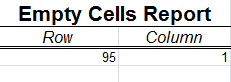
\includegraphics{MasterEmptyCellReport}
        \end{figure}
        \newline
        In the first part of the spreadsheet is the error report specifically for empty cells. If there are any empty cells within the `Data Table' spreadsheet, the macro will pick them up and output the row and column number of that cell.
        \begin{figure}[h]
        \centering
        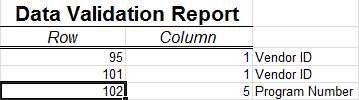
\includegraphics{MasterValidationReport}
        \end{figure}
        \newline
        In the next part is the validation report. Five columns in the `Data Table' spreadsheet are required to undergo a validation test. Any cells within those five columns that do not meet a certain requirement will be displayed in the error report in this spreadsheet with the row and column number. In addition, the name of the column will be shown adjacent to the outputted row and column.
        \subsection{Data Table Copy}
        This spreadsheet is mainly used for testing purposes from the developer side. Whenever a change needs to be made to a macro it is first tested in this spreadsheet before implementing the changes on the primary sheet.
        \subsection{DataFile Location}
        The ‘DataFile Location’ spreadsheet keeps the location of two folders and one file name being used by its macros. 
        \newline
        \newline
        In the first cell, A1, is the folder location of the user template data. A macro uses this cell to retrieve the folder path and access the user template within. If the location of the user template was changed then this cell will have to be updated in response. 
        \newline
        \newline
        In the second cell, A2, is the temporary name of the user template that needs to be accessed for importing. If any changes are made to the user template file name then this cell will need to be changed as well. The file extension is not needed for the cell.
        \newline
        \newline
        In the third cell, A3, is the folder location of where the final ASCII file will be saved. This is the file that will be uploaded to the oracle database. If the folder location of the final ASCII file needs to be changed, then simply change this contents of this cell to the new location. Inside this folder is also where the Master workbook is located, but changing the contents of this cell will not change the location of where this Master workbook will be saved.
        
        \subsection{Email Recipients}
        
        The email recipient’s spreadsheet is used by the macro that sends the error report to a list of users. That macro grabs the list of emails within this spreadsheet and emails the final error report to that list. 
        \newline
        \newline
        If any emails have to be removed, updated or added, then refrain from leaving any blank cells between emails. The macro runs through the column and stops at a blank cell. If there are blank cells between emails then the macro will not pick up any additional emails after that blank cell.

\chapter{Data Import Macro}
    \section{Description}
    Upon changes to the user data template, validation checks must occur. The validation macro is located in the master workbook to assure security. In order for the data to be passed through the macro and validated, a macro was developed to copy the contents of the user template and import the selected data into the master workbook.
    
    \section{How It Works - Technical Details}
    For ease of use a button was placed at the beginning (top-left most part) of the first sheet, Data Table. This button, labeled “Import Data”, runs the module named ImportData( ).
    \newline
    \newline
    This module assigns the active, master, workbook to a variable wbThis to determine the location of where the new data will be imported into. The user data template is opened from the file location specified inside the DataFile Location sheet and set to wbTarget to identify the target workbook from which the data will be imported. 
    \newline
    \newline
    A range is then specified, selected and then copied within the module; this is hardcoded but can be changed to be dynamic. Lastly, wbThis is reopened and the updated data is pasted starting at the specified cell. 

\chapter{Validation Macro}
    \section{Description}
    
    The main purpose of the Master workbook is to validate the updates from the user data template. Once the new data has been imported the validation process can now begin. In the next section you will find the validation requirements for the new data.
    
    \section{Validation Requirements}
        \begin{center}
        	\begin{tabular}{| c || c | c | c | p{4.5cm} |}
        	\hline
        	No & Field name & Mandatory & Length & Note \\ 
        	\hline
        	\hline
        	1 & Vendor ID &	Yes & 10 characters & Macro should preserve the leading zeros. Must be 10 characters. \\ 
        	\hline
        	2 & Program No. & Yes & 7 characters & Macro should preserve the leading zeros. Must be 7 characters. \\ 
        	\hline
        	3 & ACCIS ID & Yes & 5 characters & Macro should preserve the leading zeros. Must be 5 characters. \\ 
        	\hline
        	4 & City Lease & Optional & 3 characters & Possible values: Yes or No or Empty. \\
            \hline
        	5 & Contract No. & Yes & 11 characters & Macro should preserve the leading zeros. Must be 11 characters. \\ 
        	\hline
        	\end{tabular}
        \end{center}
    
        \subsection{Extra Notes}
        \subsubsection{City Lease}
        
        \begin{itemize}
        		\item If the original spreadsheet says Y, macro should translate it to Yes 
        		\item If the original spreadsheet says N, macro should translate it to No.
        		\item If the original spreadsheet says `Yes' or `No'; macro should copy as such. 
        	\end{itemize} 
        
    \section{How It Works}
    
    To initiate the validation of the imported data, a button was placed in the beginning (top-left most part) of the first sheet, `Data Table', labeled `Validate Text/Save to ASC/Email Errors'. To elaborate, this button will run the validation macro that will be discussed here, the conversion macro, and the emailed error report macro, which will both be discussed in later sections.
    
        \subsection{Empty Cells}
        
        Upon clicking the button, the macro named FindEmptyCells( ) will execute. Before any computations are executed, though, the sheet `EmptyCells' is cleared to start a fresh error report.
        \newline
        \newline
        A for loop is used to loop through the mandatory columns which were mentioned in the previous section. The loop in this module selects any cell that has no value inside of it and fills it with a red background in order to make it easier for locating the errors once the script finishes. 
        \newline
        \begin{figure}[h]
        \centering
        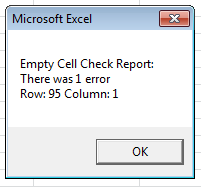
\includegraphics{MasterEmptyCellMsgbox}
        \end{figure}
        \newline
        As the loop is running and potentially picking up empty cells, the report in the next sheet `EmptyCells' gets updated with the specific row and column number of the found issue. Then, at the end of the loop, a msgbox appears with the accumulated error report. The string variable containing the message is sent over to the next macro to append to the data validation report.
        
        \subsection{Data Validation}
        
        At the end of the FindEmptyCells( ) macro, ValidateFields(String), is called; this is the module responsible for validating the imported data based upon the previous table.
        \newline
        \newline
        Within this module are five similar for loops, one for each column that needs validating: VendorID, ContractID, ACCIS, Program#, and City Lease. Following the provided table of necessary validations, the for loops run chronologically through each of the five columns. 
        \newline
        \newline
        As in the previous FindEmptyCells( ) macro, the errors are instantaneously placed in the sheet `EmptyCells'. The information provided in the validation report is similarly the row and column number, while also mentioning what the name of the column is. 
        \newline
        \begin{figure}[h]
        \centering
        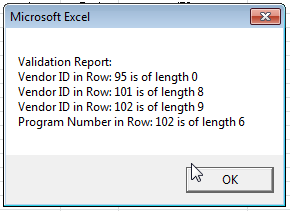
\includegraphics{MasterValidationMsgbox}
        \end{figure}
        \newline
        At the conclusion of the script a msgbox will appear presenting the found errors. The string that contains the potential errors from the validation script is appended to the string containing the error report from the last module to form one error report message. The variable finalMsg, which is holding the two appended error reports, is a publicly declared variable so it can be used by any macro within that module.


\chapter{ASCII Conversion and Email Macro}
   \section{XLS to ASCII Conversion}
   \subsection{Description}
    Once new data is imported and validated the next macro runs, CreateCSV ( ), in order to save the data as a pipe-delimited ASCII file.
    \newline
    \newline
    File Naming Convention: VERP\_BUDGET\_DATA\_YYYYMMDDHHMMSS.asc
    \subsubsection{Pre-Requirements}
    Before the data is converted, some pre-requirements have to be met.
        \begin{itemize}
            \item Formulas must be removed from all cells. Only the values should be retained.
            \item All \$ symbols should be removed.
            \item Round \$ amounts to two digits after decimal.
            \item Remove any empty columns
            \item Remove any filters applied.
            \item Remove first two rows (one with column numbers and second with merged field headings). The third row with column headers (row 3) shall be retained.
        \end{itemize}
    \subsection{How It Works - Technical Details}
    When this macro is called, initially it tries to open a file that is not there, thus creating a new file by the above file naming convention. The location of where this file will be saved to is located within the DataFile Location sheet.
    \newline
    \newline
    Since the file is required to be pipe delimited, the delimiter was hard coded into the macro. If the delimiter ever needs to be changed for future purposes, it would need to be changed in the macro itself. If for whatever reason the delimiter needs to be changed frequently, and changing it in the code becomes non-efficient, a developer could make the macro read the delimiter from a cell within a spreadsheet. Therefore, a user could change the delimiter from one of the sheets, or a new sheet, without having to access the macro.
    \newline
    \newline
    The last row is set using the 6th column due to potential of problems if row chosen was one that needed to be validated. Two nested for loops run through all rows and columns and output the cell contents into the newly created ASCII file. The pipe-delimiter is attached to the end of the cell content, unless the row equals the last row. The file is then closed and the next macro is called with a parameter of the file name of the file that was just created.
    \section{Email Error Report Macro}
    \subsection{Description}
    
    Upon completion of the validation and exportation of data to an ASCII file, the accumulated error report is then sent out, along with the ASCII file, to a list of recipients.
    
    \subsection{How It Works - Technical Details}

    This macro takes in a string parameter of the file name of the file that was created in the previous macro. The contents of the email are set as variables prior to configuration to allow easier future change.
    \newline
    \newline
    Next, the SMTP server information and CDO objects are configured according to provided information. Finally, the main options associated with emailing from a macro are initialized to the variables that were set earlier. 


\end{document}